% questions.tex —— 2004 年·全国卷Ⅰ·理科 · 题目内容片段（无答案）
% 由 tools/generate_projects.py 依来源总账自 2004/2004_数学真题_全国1理_试题.md 生成，勿手改（改源 MD 后重跑）


\gkpart{数学}

\begin{gktip}
\textbf{来源说明}：本题面依据固定源 PDF 两页 A3 题面逐题转录，原卷印刷页码 182–183。固定源不附答案，答案和解析均由本库独立复算。

\textbf{图形说明}：第 20 题的原卷图形关系重绘为 TikZ/PGFPlots 矢量图。图形标记所指的 PNG 不随仓库保存。
\end{gktip}

\gkpart{一、选择题}

\begin{question}
\gkti{1}$(1-i)^2\cdot i=$\mbox{（　　）}

（A）$2-2i$　　（B）$2+2i$　　（C）$-2$　　（D）$2$

\end{question}
\begin{question}
\gkti{2}已知函数 $f(x)=\lg\dfrac{1-x}{1+x}$，若 $f(a)=b$，则 $f(-a)=$\mbox{（　　）}

（A）$b$　　（B）$-b$　　（C）$\dfrac1b$　　（D）$-\dfrac1b$

\end{question}
\begin{question}
\gkti{3}已知 $\boldsymbol a\text{、}\boldsymbol b$ 均为单位向量，它们的夹角为 $60^\circ$，那么 $|\boldsymbol a+3\boldsymbol b|=$\mbox{（　　）}

（A）$\sqrt7$　　（B）$\sqrt{10}$　　（C）$\sqrt{13}$　　（D）$4$

\end{question}
\begin{question}
\gkti{4}函数 $y=\sqrt{x-1}+1$（$x\geqslant1$）的反函数是\mbox{（　　）}

（A）$y=x^2-2x+2$（$x<1$）　　（B）$y=x^2-2x+2$（$x\geqslant1$）

（C）$y=x^2-2x$（$x<1$）　　（D）$y=x^2-2x$（$x\geqslant1$）

\end{question}
\begin{question}
\gkti{5}$\left(2x^3-\dfrac1{\sqrt{x}}\right)^7$ 的展开式中常数项是\mbox{（　　）}

（A）$14$　　（B）$-14$　　（C）$42$　　（D）$-42$

\end{question}
\begin{question}
\gkti{6}设 $A\text{、}B\text{、}I$ 均为非空集合，且满足 $A\subseteq B\subseteq I$，则下列各式中错误的是\mbox{（　　）}

（A）$(\complement_I A)\cup B=I$　　（B）$(\complement_I A)\cup(\complement_I B)=I$

（C）$A\cap(\complement_I B)=\varnothing$　　（D）$(\complement_I A)\cap(\complement_I B)=\complement_I B$

\end{question}
\begin{question}
\gkti{7}椭圆 $\dfrac{x^2}{4}+y^2=1$ 的两个焦点为 $F_1\text{、}F_2$，过 $F_1$ 作垂直于 $x$ 轴的直线与椭圆相交，一个交点为 $P$，则 $|\overline{PF_2}|=$\mbox{（　　）}

（A）$\dfrac{\sqrt3}{2}$　　（B）$\sqrt3$　　（C）$\dfrac72$　　（D）$4$

\end{question}
\begin{question}
\gkti{8}设抛物线 $y^2=8x$ 的准线与 $x$ 轴交于点 $Q$，若过点 $Q$ 的直线 $l$ 与抛物线有公共点，则直线 $l$ 的斜率的取值范围是\mbox{（　　）}

（A）$\left[-\dfrac12,\dfrac12\right]$　　（B）$[-2,2]$　　（C）$[-1,1]$　　（D）$[-4,4]$

\end{question}
\begin{question}
\gkti{9}为了得到函数 $y=\sin\left(2x-\dfrac\pi6\right)$ 的图象，可以将函数 $y=\cos2x$ 的图象\mbox{（　　）}

（A）向右平移 $\dfrac\pi6$ 个单位长度　　（B）向右平移 $\dfrac\pi3$ 个单位长度

（C）向左平移 $\dfrac\pi6$ 个单位长度　　（D）向左平移 $\dfrac\pi3$ 个单位长度

\end{question}
\begin{question}
\gkti{10}已知正四面体 $ABCD$ 的表面积为 $S$，其四个面的中心分别为 $E\text{、}F\text{、}G\text{、}H$。设四面体 $EFGH$ 的表面积为 $T$，则 $\dfrac TS$ 等于\mbox{（　　）}

（A）$\dfrac19$　　（B）$\dfrac49$　　（C）$\dfrac14$　　（D）$\dfrac13$

\end{question}
\begin{question}
\gkti{11}从数字 $1,2,3,4,5$ 中，随机抽取 3 个数字（允许重复）组成一个三位数，其各位数字之和等于 9 的概率为\mbox{（　　）}

（A）$\dfrac{13}{125}$　　（B）$\dfrac{16}{125}$　　（C）$\dfrac{18}{125}$　　（D）$\dfrac{19}{125}$

\end{question}
\begin{question}
\gkti{12}$a^2+b^2=1$，$b^2+c^2=2$，$c^2+a^2=2$，则 $ab+bc+ca$ 的最小值为\mbox{（　　）}

（A）$\sqrt3-\dfrac12$　　（B）$\dfrac12-\sqrt3$　　（C）$-\dfrac12-\sqrt3$　　（D）$\dfrac12+\sqrt3$

\end{question}
\gkpart{二、填空题}

\begin{question}
\gkti{13}不等式 $|x+2|\geqslant|x|$ 的解集是\gkblank{}。

\end{question}
\begin{question}
\gkti{14}由动点 $P$ 向圆 $x^2+y^2=1$ 引两条切线 $PA\text{、}PB$，切点分别为 $A\text{、}B$，$\angle APB=60^\circ$，则动点 $P$ 的轨迹方程为\gkblank{}。

\end{question}
\begin{question}
\gkti{15}已知数列 $\{a_n\}$，满足 $a_1=1$，

\nopagebreak[4]
\[
a_n=a_1+2a_2+3a_3+\cdots+(n-1)a_{n-1}\quad(n\geqslant2)\text{，}
\]

\Needspace{5\baselineskip}
则 $\{a_n\}$ 的通项 $a_n=$

\nopagebreak[4]
\[
\begin{cases}
1,&n=1,\\
\rule{3em}{0.4pt},&n\geqslant2.
\end{cases}
\]

\end{question}
\begin{question}
\gkti{16}已知 $\boldsymbol a\text{、}\boldsymbol b$ 为不垂直的异面直线，$\alpha$ 是一个平面，则 $\boldsymbol a\text{、}\boldsymbol b$ 在 $\alpha$ 上的射影有可能是：

① 两条平行直线；

② 两条互相垂直的直线；

③ 同一条直线；

④ 一条直线及其外一点。

在上面结论中，正确结论的编号是\gkblank{}。（写出所有正确结论的编号）

\end{question}
\gkpart{三、解答题}

\begin{question}
\gkti{17}求函数

\nopagebreak[4]
\[
f(x)=\frac{\sin^4x+\cos^4x+\sin^2x\cos^2x}{2-\sin2x}
\]

的最小正周期、最大值和最小值。

\end{question}
\begin{question}
\gkti{18}一接待中心有 $A\text{、}B\text{、}C\text{、}D$ 四部热线电话，已知某一时刻电话 $A\text{、}B$ 占线的概率均为 $0.5$，电话 $C\text{、}D$ 占线的概率均为 $0.4$，各部电话是否占线相互之间没有影响。假设该时刻有 $\xi$ 部电话占线。试求随机变量 $\xi$ 的概率分布和它的期望。

\end{question}
\begin{question}
\gkti{19}已知 $a\in\mathbb R$，求函数 $f(x)=x^2e^{ax}$ 的单调区间。

\Needspace{0.4\textheight}
\end{question}
\begin{question}
\gkti{20}如图，已知四棱锥 $P-ABCD$，$PB\perp AD$，侧面 $PAD$ 为边长等于 2 的正三角形，底面 $ABCD$ 为菱形，侧面 $PAD$ 与底面 $ABCD$ 所成的二面角为 $120^\circ$。
\nopagebreak[4]
\begin{center}% 2004 年全国卷Ⅰ理科第 20 题：四棱锥
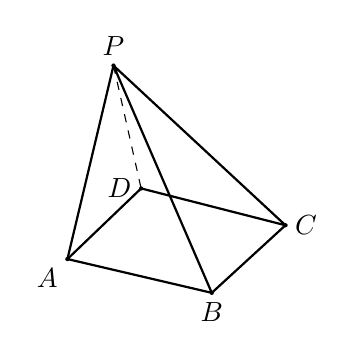
\begin{tikzpicture}[>=stealth,scale=0.78]
  \coordinate (A) at (0,0); \coordinate (B) at (2.35,-0.55);
  \coordinate (C) at (3.55,0.55); \coordinate (D) at (1.2,1.15);
  \coordinate (P) at (0.75,3.15);
  \draw[thick] (A)--(B)--(C)--(D)--cycle;
  \draw[thick] (P)--(A) (P)--(B) (P)--(C);
  \draw[dashed] (P)--(D);
  \fill (P) circle (1pt) node[above] {$P$};
  \fill (A) circle (1pt) node[below left] {$A$};
  \fill (B) circle (1pt) node[below] {$B$};
  \fill (C) circle (1pt) node[right] {$C$};
  \fill (D) circle (1pt) node[left] {$D$};
\end{tikzpicture}
\end{center}
\nopagebreak[4]
（1） 求点 $P$ 到平面 $ABCD$ 的距离；

（2） 求面 $APB$ 与面 $CPB$ 所成二面角的大小。

\end{question}
\begin{question}
\gkti{21}已知双曲线 $C:\dfrac{x^2}{a^2}-y^2=1$（$a>0$）与直线 $l:x+y=1$ 相交于两个不同的点 $A\text{、}B$。

（1） 求双曲线 $C$ 的离心率 $e$ 的取值范围；

（2） 设直线 $l$ 与 $y$ 轴的交点为 $P$，且 $\overrightarrow{PA}=\dfrac5{12}\overrightarrow{PB}$。求 $a$ 的值。

\end{question}
\begin{question}
\gkti{22}已知数列 $\{a_n\}$ 中，$a_1=1$，且

\nopagebreak[4]
\[
a_{2k}=a_{2k-1}+(-1)^k,\qquad a_{2k+1}=a_{2k}+3^k,\qquad k=1,2,3,\cdots\text{。}
\]

（1） 求 $a_3\text{、}a_5$；

（2） 求 $\{a_n\}$ 的通项公式。

\end{question}